% Created 2018-04-16 Mon 16:59
% Intended LaTeX compiler: pdflatex
\documentclass[11pt]{article}
\usepackage[utf8]{inputenc}
\usepackage[T1]{fontenc}
\usepackage{graphicx}
\usepackage{grffile}
\usepackage{longtable}
\usepackage{wrapfig}
\usepackage{rotating}
\usepackage[normalem]{ulem}
\usepackage{amsmath}
\usepackage{textcomp}
\usepackage{amssymb}
\usepackage{capt-of}
\usepackage{hyperref}
\date{\today}
\title{OpenCV workshop project: How many triangles do you see?}
\hypersetup{
 pdfauthor={Mehran Pesteie},
 pdftitle={OpenCV workshop project: How many triangles do you see?},
 pdfkeywords={},
 pdfsubject={},
 pdfcreator={Emacs 25.1.1 (Org mode 9.1.2)}, 
 pdflang={English}}
\begin{document}

\maketitle

\section{What}
\label{sec:org275de49}
One of the riddles that basically divided the internet was the one that was posted on People's Daily China twitter account (\href{https://twitter.com/PDChina/status/806615066133090308/photo/1?ref\_src=twsrc\%255Etfw\&ref\_url=https\%253A\%252F\%252Fwww.telegraph.co.uk\%252Fnews\%252F2016\%252F12\%252F08\%252Fmany-triangles-can-see-puzzle-divides-internet\%252F}{Click here to see the post}).
It simply asks how many triangles are in the following image:
\begin{center}
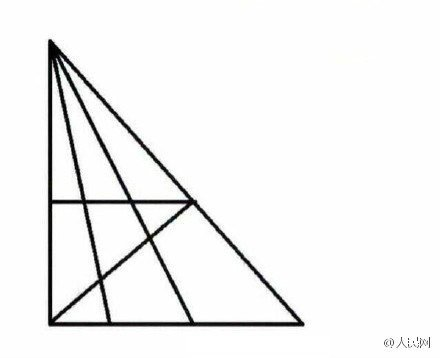
\includegraphics[width=.9\linewidth]{./final.jpeg}
\end{center}

For the final project of the workshop, write a function in python and OpenCV that returns the number of triangles in this image. You can use any computer vision algorithm that you wish.

\section{How}
\label{sec:org81d343a}
Your function should have the following prototype:

\begin{verbatim}
def count_triangles(image):
count = 0
...
return count 
\end{verbatim}

Save your function in a file called 'solution.py' and put it in a zip file along with your document.
Send your zip file to mehranp@ece.ubc.ca

\section{When}
\label{sec:org290b5db}
April 20, 2018 11:59 PST
\end{document}